\chapter{Development Methodology}

\textcolor{red}{\textbf{TODO: Possibly restructure this, it\'s a start for now. Not 100\% sure what Neil\'s looking for here.}}

\section{Initial Project Plan}
\par
At the start of the project the group met and decided on a standard style of development which would be most suitable for the project. After some discussion, we agreed to adopt the \textit{Scrumban}\cite{scrumban} methodology. 

\par
As this project has a relatively short deadline with a team consisting of only eight developers we adopted Scrumban, which focuses on flexibility and adaptability for both the project's plan and sprints. 
The team had no prior development experience with the application stacks we were required to use, Java EE and .NET Core. \textit{Scrumban} is tailored for the difficulties around estimating each sprint or the current velocity.

\par
The application's requirements were initially broken down into nine distinct microservices. The group then discussed which language to use for each service. (Fig. \ref{fig:initial_spec_chart})

\begin{figure}[H]
    \centering
    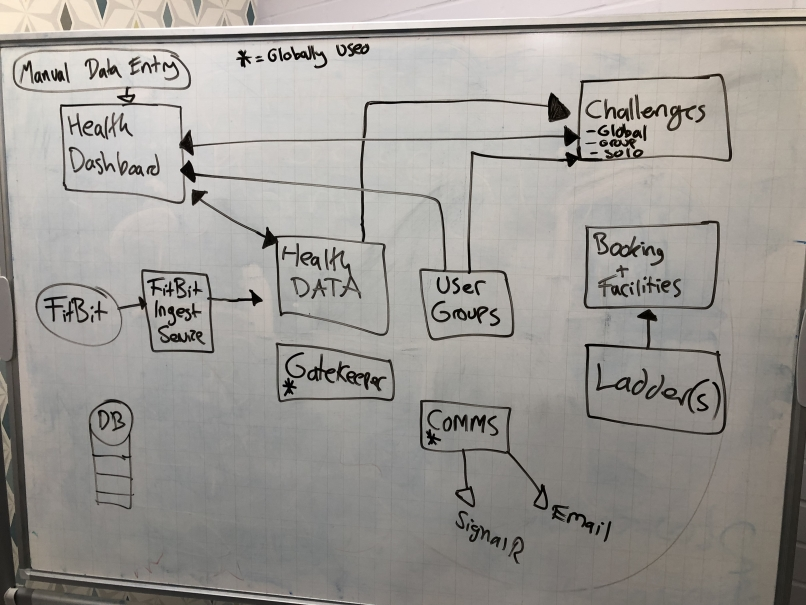
\includegraphics[width=\textwidth]{Images/Initial_Spec_Chart.jpg}
    \caption{An initial design diagram which was used to break the project down into smaller microservices and their interactions with each other}
    \label{fig:initial_spec_chart}
\end{figure}

\par
We proceeded to allocate each microservice to two developer teams, then assigned each service a priority ranking between 1 and 3. Core services were marked with a priority of 1, as many other parts of the \textit{AberFitness} infrastructure heavily relied on their APIs in order to function correctly. One examples is the \textit{Health Data Repository} which centrally stores users' activity data. (Fig. \ref{fig:numbering_microservice_priority})

\begin{figure}[H]
    \centering
    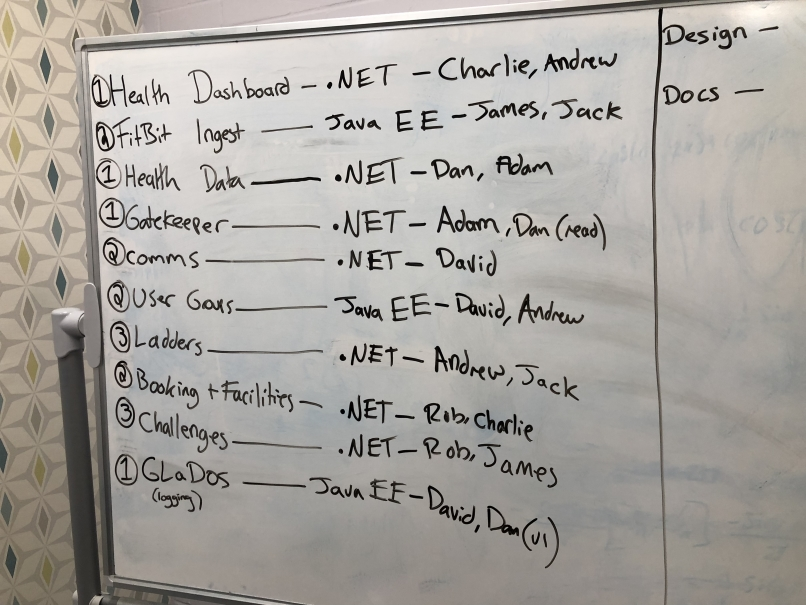
\includegraphics[width=\textwidth]{Images/Numbering_Microservices.jpg}
    \caption{Initial plan for microservices priorities and allocation to developers}
    \label{fig:numbering_microservice_priority}
\end{figure}


\section{Supporting Tools}
\subsection{GitHub \& TravisCI}
The source control for \textit{Aber Fitness} is hosted on \textit{GitHub}\footnote{https://github.com/sem5640-2018}. \textit{GitHub} provides multiple features that were incredibly useful during the development phase. This included native integration with \textit{Slack} for notifications straight to the respective development channels. The git flow was complemented with \textit{TravisCI} to automatically trigger unit tests and \textit{Docker} image builds. We also developed a development pattern of requiring all code to be peer reviewed through the use of pull requests and branch protection.

\par
Branch protection is a collection of conditions which must be met before a pull request can be merged into \textit{development} or \textit{master} branches. We configured branch protection in order to ensure that only tested, peer reviewed code would be committed. This reduced the likelihood of new bugs being introduced and ensured code quality was maintained.

\begin{figure}[H]
    \centering
    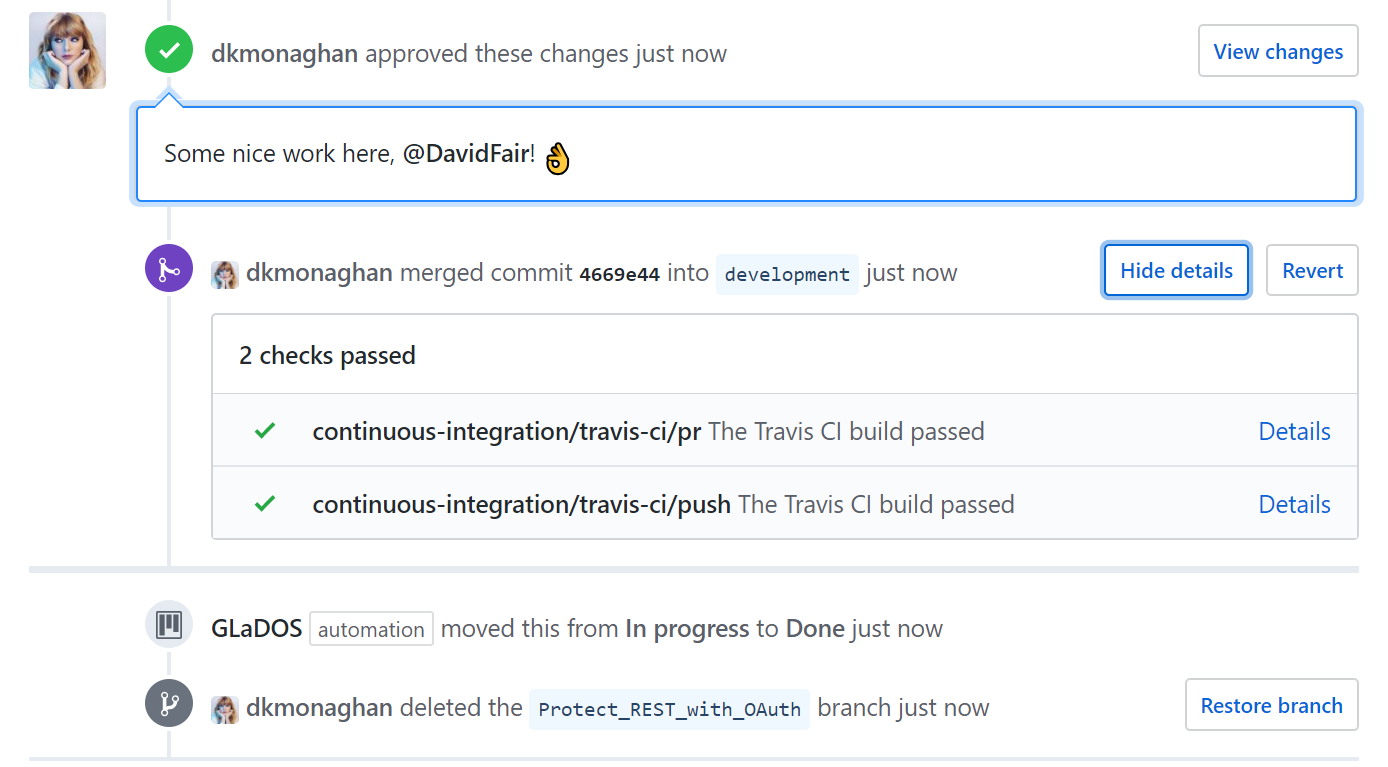
\includegraphics[width=\textwidth]{Images/approve_pr.png}
    \caption{A screenshot showing a pull request on the \textit{GLaDOS} repository being peer reviewed. The continuous integration checks run on \textit{TravisCI} have completed allowing the branch to merge into an upstream branch.}
    \label{fig:approve_pull_request}
\end{figure}

\par
Once a pull request had been approved and merged (Fig. \ref{fig:approve_pull_request}), \textit{TravisCI} would then build and push the \textit{Docker} image to \textit{Docker Hub}.

\begin{figure}[H]
    \centering
    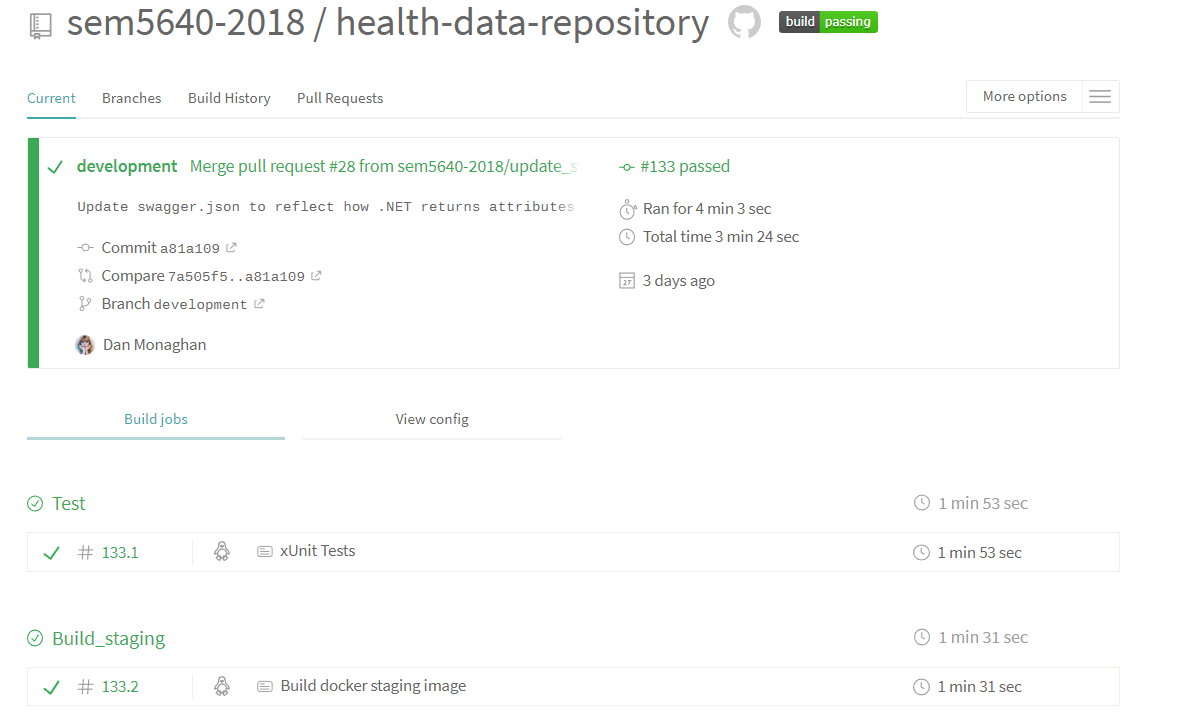
\includegraphics[width=\textwidth]{Images/travis_builds_overview.png}
    \caption{A screenshot from \textit{TravisCI} demonstrating a pull request being merged into the \textit{development} branch. This runs the unit tests and then building the \textit{Docker} image}
    \label{fig:travis_ui}
\end{figure}

\subsection{Swagger}
\begin{figure}[H]
    \centering
    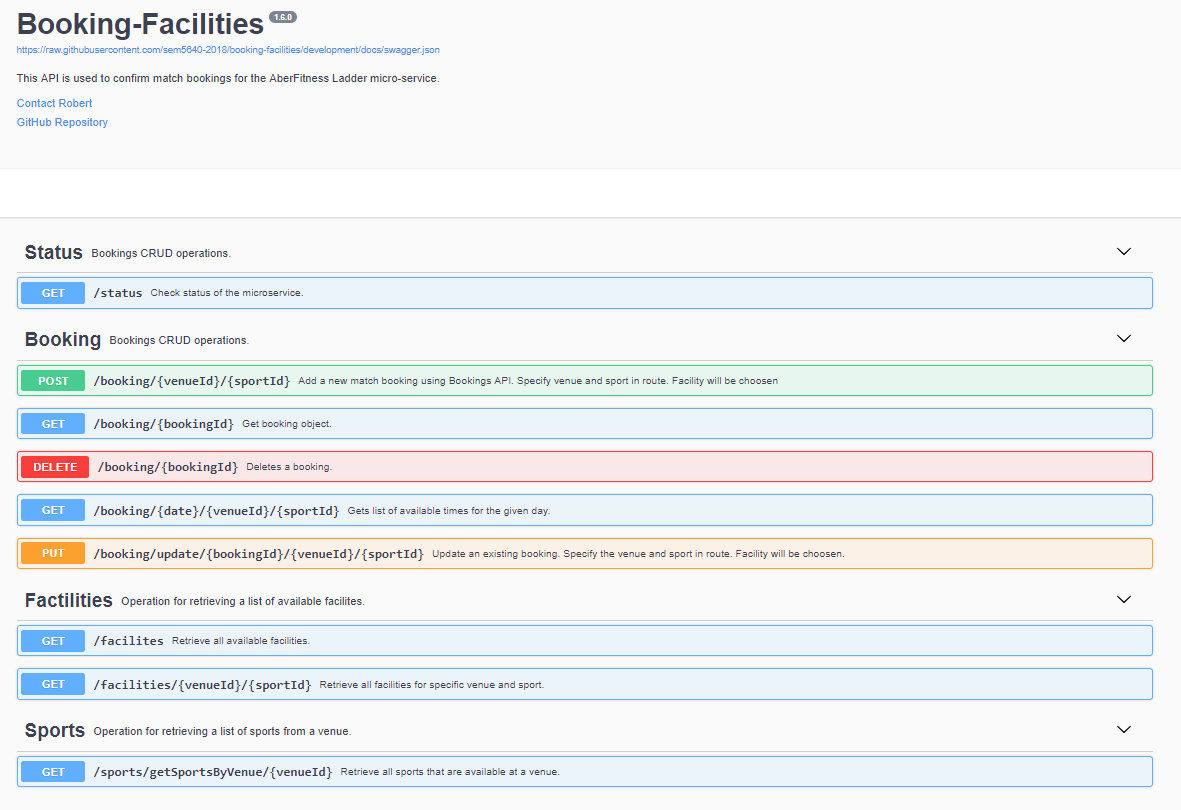
\includegraphics[width=\textwidth]{Images/Swagger.png}
    \caption{The Swagger interface for the \textit{Booking Facilities} microservice}
    \label{fig:swagger_ui}
\end{figure}

\par
\textit{Swagger} is a web based application for documenting API specifications. Each microservice within \textit{Aber Fitness} has a file located in \lstinline{docs/swagger.json} which defines its API endpoints and any associated data models. \textit{Swagger} was a crucial part of the development process as it allowed us to draft API specifications. Other members of the group could give feedback and identify issues before commencing development. 


\subsection{Portainer}
\begin{figure}[H]
    \centering
    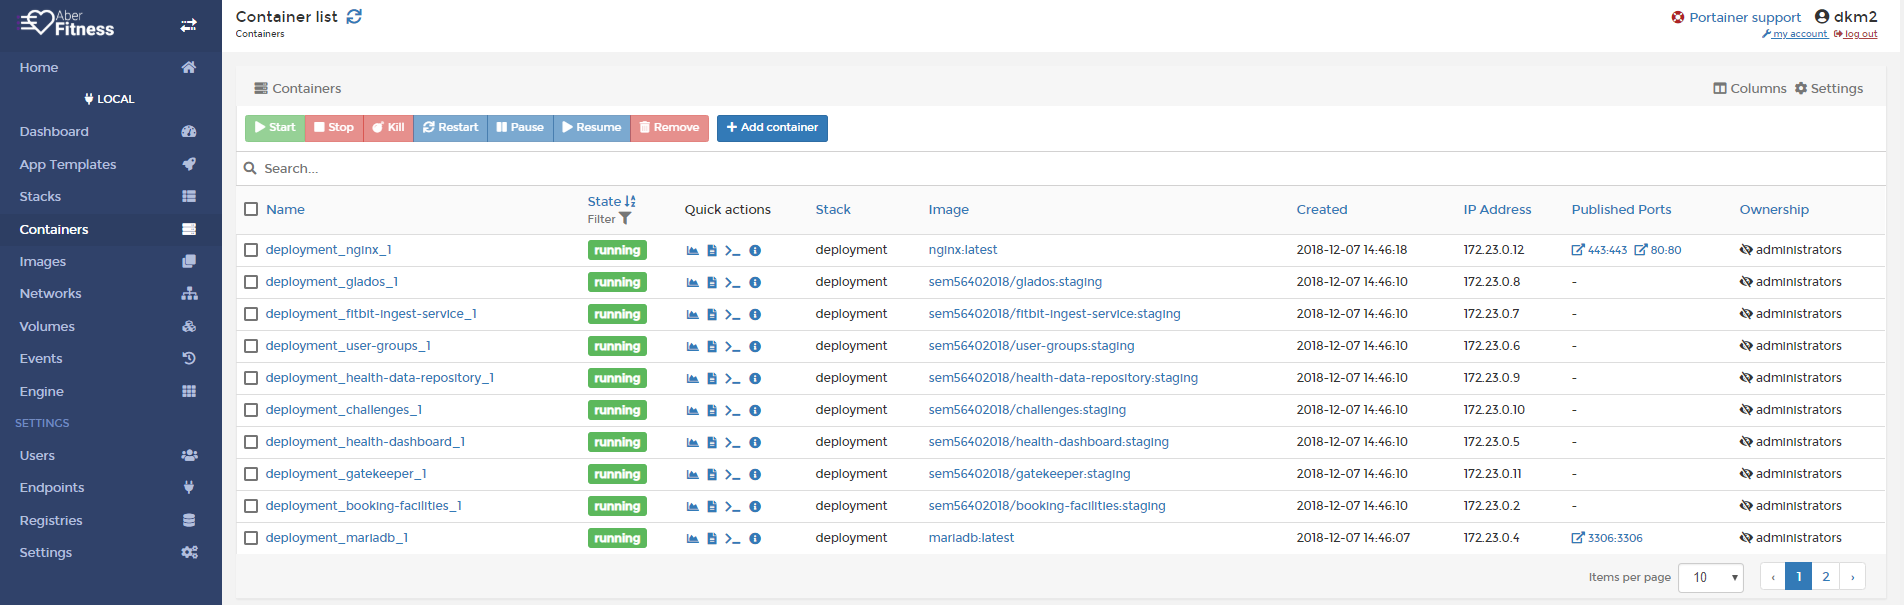
\includegraphics[width=\textwidth]{Images/Portainer.png}
    \caption{The Portainer interface for our staging / development Docker host, \lstinline{docker2-m56.dcs.aber.ac.uk}}
    \label{fig:portainer_ui}
\end{figure}

\par
\textit{Portainer} provides a dashboard for managing \textit{Docker} volumes, networks, images and containers. Whilst completing the initial configuration of the \textit{Docker} images, \textit{Portainer} proved invaluable, it provided rapid visual feedback allowing developers to quickly and easily understand what the host was running. \textbf{TODO: More here probably.}

\subsection{Docker Hub}
\par
\textit{Docker Hub} is an online platform provided by \textit{Docker} which allows \textit{Docker} container images to be uploaded and hosted. The image full system stack is defined in the \lstinline{docker-compose} file, which can be updated and re-deployed . As part of our build process (Fig. \ref{fig:development_flow_diagram}), images are built by \textit{TravisCI} and then pushed to \textit{Docker Hub} before being pulled down onto the \textit{Docker} hosts.


\subsection{Slack \& Deployment}
\par
\textit{Slack} is a hosted chat service designed for offices and teams, and particularly suits itself to the development of software. The group used \textit{Slack} extensively throughout the development of \textit{Aber Fitness} not only to communicate and discuss progress, ideas and troubleshoot problems, but also made extensive use of \textit{Slack}'s integrations with services such as \textit{TravisCI} and \textit{GitHub} (Fig. \ref{fig:slack_travis_github})

\begin{figure}[H]
    \centering
    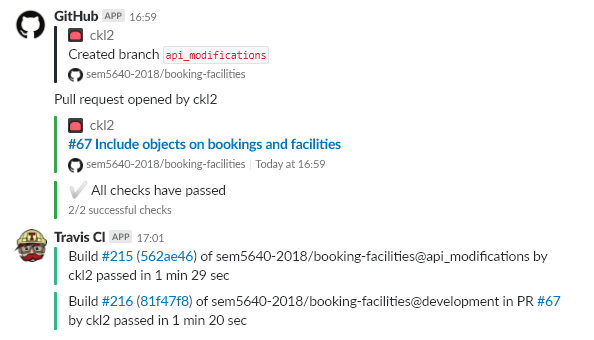
\includegraphics[width=\textwidth]{Images/Slack_Travis_GitHub.png}
    \caption{A screenshot of the \textit{Slack} channel \lstinline{\#dev-booking-facilities} demonstrating the integrations between \textit{Slack}, \textit{GitHub} and \textit{TravisCI}}
    \label{fig:slack_travis_github}
\end{figure}

\par
\textit{Slack} also played a major role in our deployment strategy when rolling out updated \textit{Docker} images to our staging host. On multiple occasions we ran into permission issues whilst trying to deploy on the two \textit{Docker} hosts we had been provided by the Computer Science department. Each member of the team had their own individual login to the hosts, so permissions errors would occur after performing commands like \lstinline{git pull}. 

\par
Another issue we ran into was developers forgetting the specific command sequence to update the application images. This would lead to confusion when the upstream changes were not deployed, wasting valuable development time resolving bugs. (Fig. \ref{fig:david_being_a_dumbass})

\begin{figure}[H]
    \centering
    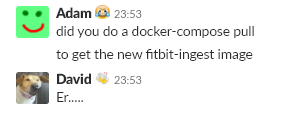
\includegraphics[width=0.5\textwidth]{Images/aberfitness_slack_bot_reason_why.png}
    \caption{An example situation where the execution of \lstinline{docker-compose pull} caused a large amount of confusion amongst \textit{Aber Fitness} developers}
    \label{fig:david_being_a_dumbass}
\end{figure}

\par
\textit{Slack} ended up providing us with an elegant solution to this, users could call a custom webhook by entering a specific command in a chat channel. A \textit{Slack} application was put together to automatically pull the latest \lstinline{docker-compose.yml} file from GitHub, as well as updating all the \textit{Docker Hub} images, then re-deploy the stack. This could all be done from within \textit{Slack} itself through the \lstinline{/deploy} command. (Fig. \ref{fig:slack_bot})

\begin{figure}[H]
    \centering
    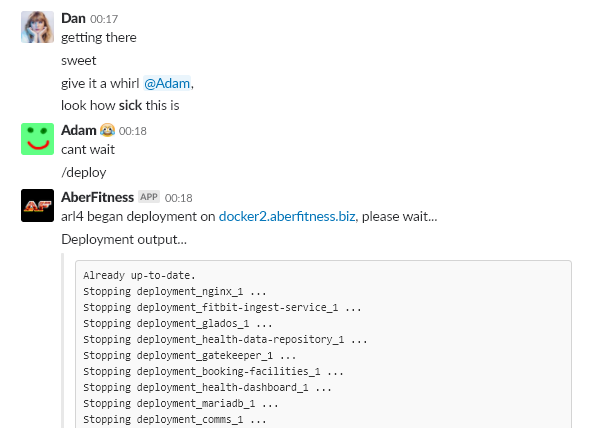
\includegraphics[width=0.9\textwidth]{Images/aberfitness_slack_bot.png}
    \caption{A demonstration of the \lstinline{/deploy} command being used to re-deploy \textit{Aber Fitness} onto the staging host}
    \label{fig:slack_bot}
\end{figure}

